\section{Complexity Analysis}

\subsection{Complexity Analysis}
\begin{frame}
    \frametitle{Serial Cache Complexity Analysis}
    \begin{itemize}
    	\item $Q_f(n)$ denote the cache complexity of $f_{par}$ on a matrix of size $n \times n$
    	\item $f \in \left\{ A, B, C \right\}$
    \end{itemize}
    \begin{align*}
		Q_f(n) &= \mathcal{O}(n + n^2 / B) 
			&& \text{if } n^2 \le \gamma_f M, \; \gamma_f \in (0, 1 ] \\
		Q_A(n) &= Q_A(n/2) + Q_B(n/2) \\
		Q_B(n) &= 4 Q_B(n/2) \\
		Q_C(n) &= 8 Q_C(n/2)
    \end{align*}
    \begin{align*}
    	&\Rightarrow Q_A(n) = \mathcal{O}\left(n + n^2/B + n^3 /M + n^3 / \left(B \sqrt{M}\right)  \right)
  	\end{align*}
\end{frame}

\begin{frame}
    \frametitle{Span Analysis}
    \begin{itemize}
    	\item $T_f(n)$ denote the span complexity of $f_{par}$ on a matrix of size $n \times n$
    	\item $f \in \left\{ A, B, C \right\}$
    \end{itemize}
    \begin{align*}
		T_f(n) &= \Theta(1)
			&& \text{if } n = 1 \\
		T_A(n) &= T_A(n/2) + T_B(n/2) + \Theta(1) \\
		T_B(n) &= 3 (T_B(n/2) + T_C(n/2)) + \Theta(1) \\
		T_C(n) &= 2 T_C(n/2) + \Theta(1)
    \end{align*}
    \begin{align*}
    	& \Rightarrow T_A(n) = \mathcal{O}\left(n^{\log_2 3}\right)
  	\end{align*}
\end{frame}

\subsection{Complexity Table}
\begin{frame}
    \frametitle{Complexity Table}
    \begin{figure}
		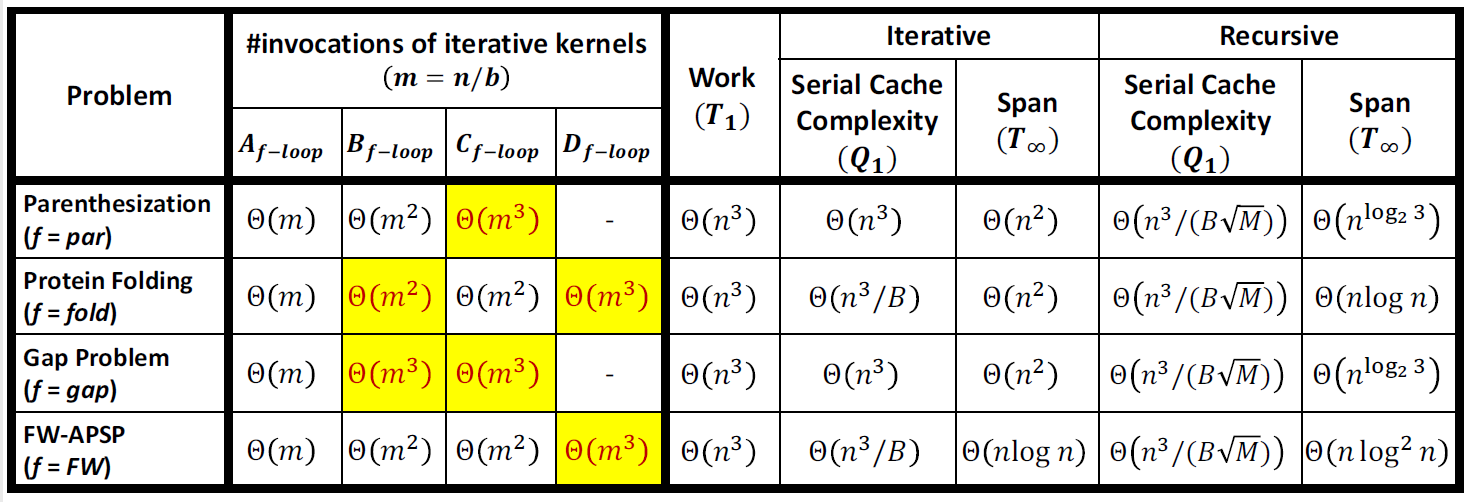
\includegraphics[scale=0.25]{figure/fig-complexity.png}
	\end{figure}
    \begin{itemize}
		\item size of cache $M$, cache line size $B$, processing elements $p$
		\item Runtime $T_p = \mathcal{O}(T_1/p + T_{\infty})$
		\item Cache complexity $Q_p = \mathcal{O}(Q_1 + p(M/B) T_{\infty})$
	\end{itemize}
\end{frame}